\documentclass[10pt]{beamer}
\usetheme{Madrid}
\usecolortheme{default}
\usepackage[T1]{fontenc}
\usepackage{lmodern}
\usepackage{graphicx}
\usepackage{booktabs}
\title{An Agent Lab for Scientific Software Optimization}
\subtitle{Deforming Bubble: FP64 to ready-to-evolve}
\author{Agent Lab}
\date{2026-10-20}

\begin{document}

\begin{frame}
\titlepage
\end{frame}

\begin{frame}{The ask}
\begin{itemize}
\item App: Deforming Bubble, level-set mini-app ported from Flash-X (WENO5 advection, redistance, MPI).
\item Scientist: ``I have added my code to the app, and ready for optimization.''
\item Agent: not yet --- optimization needs a low-precision seed, so propose \emph{raptorize}.
\item App checked against 13-point contract: all pass, natively and in Docker.
\item Plan ready 14 minutes later, every decision cited.
\end{itemize}
\end{frame}

\begin{frame}{Lab layout}
\begin{itemize}
\item \texttt{app/} swappable code (today: the bubble).
\item \texttt{dev/workflows/} general contracts: protocol, raptorize, optimize, verify.
\item \texttt{experiments/2026-10-20/}: question, runs, patches, results.
\item Stages: raptorize $\rightarrow$ optimize $\rightarrow$ verify.
\end{itemize}
\end{frame}

\begin{frame}{How it went}
\begin{itemize}
\item 17 messages, 282 scientist words; 18 min scientist time.
\item Profile: advection 52\% runtime, redistance 24\%.
\item Baseline re-run in container so ``unchanged'' compares one compiler.
\item Full run to deformation; MPI core-pinning fixed with one flag.
\item 2 MPI ranks: field bit-identical to 1 rank in all 11 frames.
\end{itemize}
\end{frame}

\begin{frame}{Results at $t=2$}
\centering
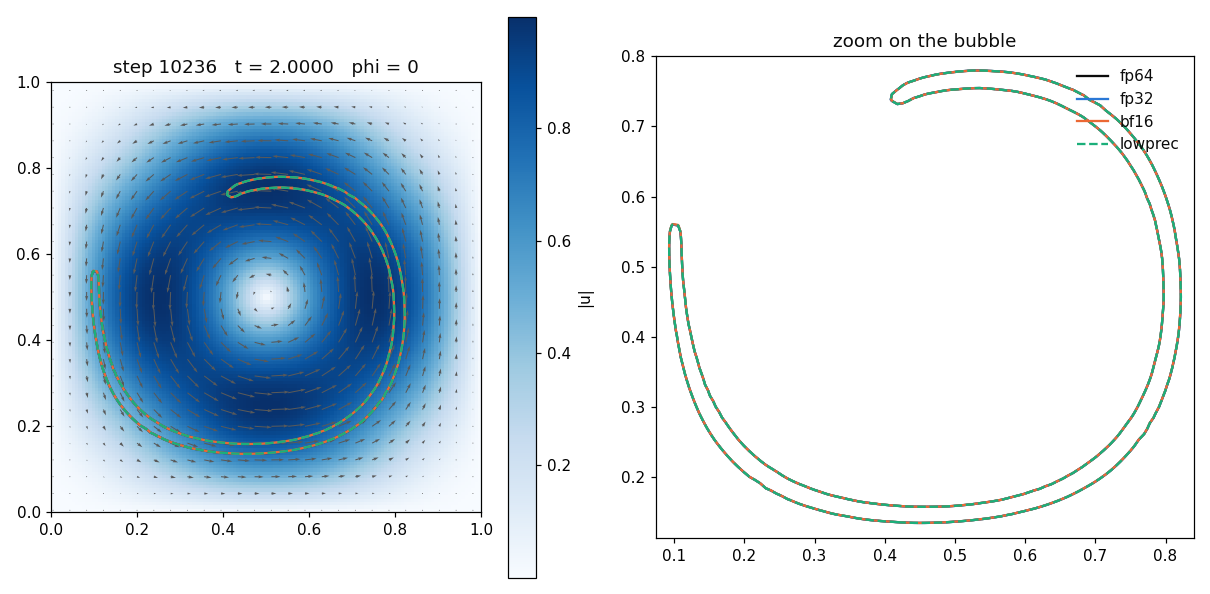
\includegraphics[width=0.95\linewidth]{figures/full_compare_010236.png}
\end{frame}

\begin{frame}{Error summary}
\begin{tabular}{@{}lll@{}}
\toprule
mode & RMS error at $t=2$ & note \\
\midrule
fp32 (emulated) & $6.3\times10^{-7}$ & 30 min emulation \\
float seed (native) & $6.3\times10^{-7}$ & same, bit for bit, 17 s \\
bf16 (emulated) & $2.6\times10^{-4}$ & 400x worse, invisible \\
\bottomrule
\end{tabular}
\vspace{0.5em}
\begin{itemize}
\item Float seed matches emulated fp32 bit for bit.
\item Error lives away from the bubble edge.
\item Hint: score near the interface in optimize.
\end{itemize}
\end{frame}

\begin{frame}{Optimize so far}
\begin{itemize}
\item Plan, evaluator, and job written.
\item Seed score: 9.2722 (twice, identical).
\item Red-team: cheats score null or below seed.
\item Launch blocked on Google Cloud credentials.
\end{itemize}
\end{frame}

\begin{frame}{Cost}
\begin{tabular}{@{}lrrr@{}}
\toprule
class & tokens & \$/M & \$ \\
\midrule
fresh input & 208 & 4.00 & 0.00 \\
cache writes & 624,107 & 5.00 & 3.12 \\
cache reads & 13,294,158 & 0.20 & 2.66 \\
output & 90,268 & 20.00 & 1.81 \\
\midrule
total & & & 7.59 \\
\bottomrule
\end{tabular}
\vspace{0.5em}
\begin{itemize}
\item 95\% of reads from cache.
\item Cache writes are the biggest line; long pauses re-cache.
\end{itemize}
\end{frame}

\begin{frame}{Human vs. agent time}
\begin{itemize}
\item By hand (expert, new to lab): $\approx$10 h.
\item With agent: 18 min scientist attention.
\item $\approx$30x reduction for \$7.59.
\item Agent worked 49 of 95 minutes.
\end{itemize}
\end{frame}

\begin{frame}{What we'd change}
\begin{itemize}
\item Keep open gates visible.
\item One-hour cache for half-hour runs.
\item Score where the physics is (interface error).
\item App should create output folder parents.
\end{itemize}
\end{frame}

\begin{frame}{Current state}
\begin{itemize}
\item \texttt{app/} restored from raptorize.patch; health checks pass.
\item Optimize calibrated (9.2722) and red-teamed.
\item Launch blocked on GCP credentials and YAML placeholders.
\end{itemize}
\end{frame}

\end{document}
